\section{Foundations of Efficiency}
Quantifying the energy demand of a vehicle begins with first principles. This section establishes a framework to understand how physical forces, design choices, and driving behavior jointly determine the energy efficiency of small personal vehicles. Starting from the classical longitudinal force balance, we derive expressions for steady-state cruising power and identify dominant energy losses. We then extend the model to incorporate real-world driving conditions idling, acceleration, braking and the embedded energy associated with mass and manufacturing. By disentangling these contributors, we identify which design decisions yield the most significant reductions in energy consumption, both during operation and over the vehicle’s full lifecycle.

\subsection{Longitudinal Dynamics: A First-Principles Approach}
The longitudinal dynamics of a ground vehicle can be expressed by Newton’s second law:

\begin{figure}[h!]
    \centering
    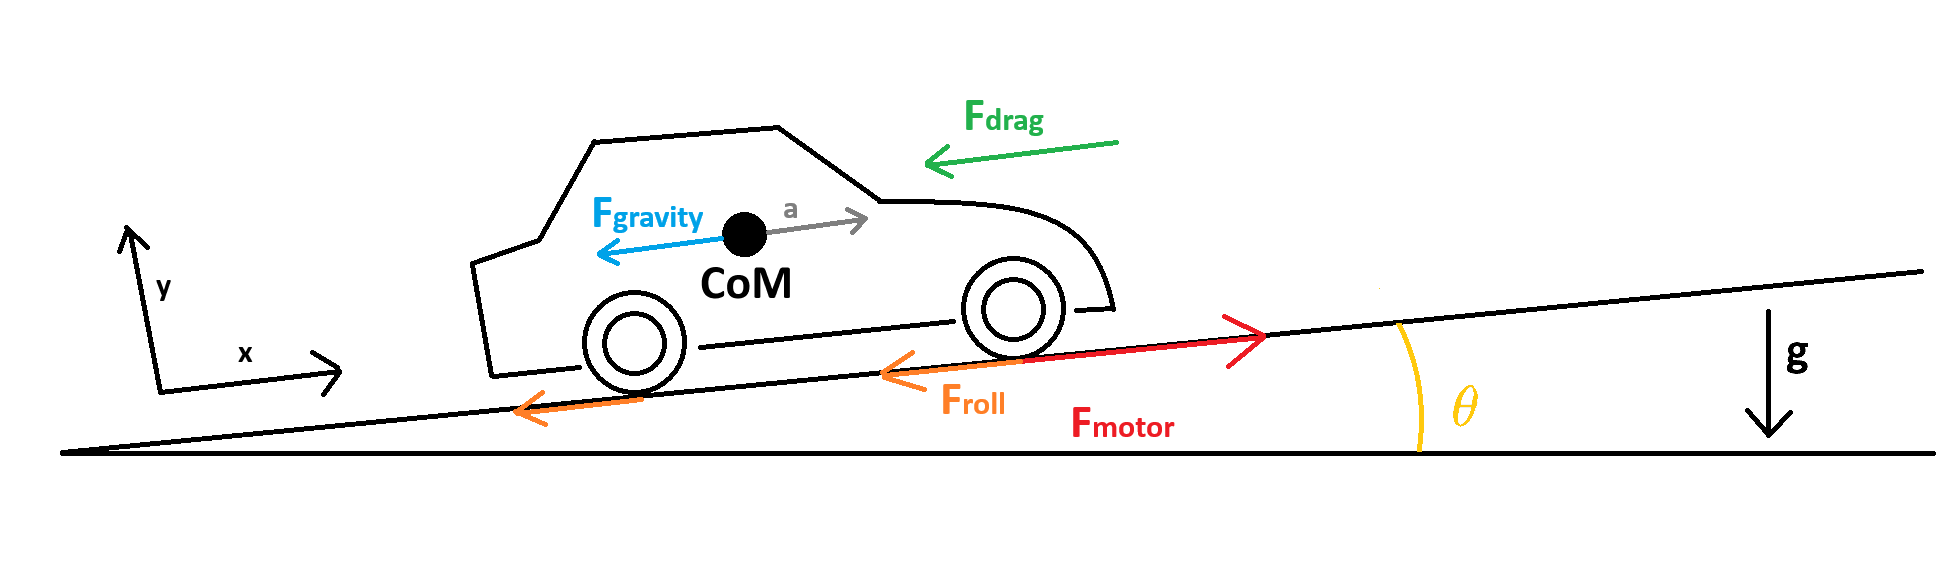
\includegraphics[width=1\linewidth]{Figures/ch1_ForceAxis.png}
    \caption{Longitudinal car dynamics}
    \label{fig:longcardynamics}
\end{figure}

To model the energy requirements of a vehicle in motion, we begin with the classical longitudinal force balance:

\[
m \cdot a = F_{\text{motor}} - F_{\text{drag}} - F_{\text{roll}} + F_{\text{gravity}}
\]

This equation expresses Newton’s second law applied to a vehicle moving along a slope, where \( m \) is the vehicle mass and \( a \) its acceleration. The right-hand side aggregates all relevant external forces acting on the vehicle in the direction of travel.

Substituting each component force into the equation, we obtain the fully expanded expression:

\[
m \cdot a = F_{\text{motor}} - \frac{1}{2} \rho\, C_d\, A\, v^2 - C_{rr}\, m\, g + m\, g\, \sin\theta
\]

This relation captures the competing effects of propulsion, aerodynamic drag, rolling resistance, and gravitation trough road slope. Each parameter affect directly energy consumption.

\vspace{0.5em}
\noindent
\textbf{Definition of Parameters:}
\begin{align*}
m &:\ \text{vehicle mass [kg]} \\
a &:\ \text{longitudinal acceleration [m/s}^2\text{]} \\
F_{\text{motor}} &:\ \text{force produced by the motor or absorbed by braking [N]} \\
\rho &:\ \text{air density [kg/m}^3\text{]} \\
C_d &:\ \text{aerodynamic drag coefficient [–]} \\
A &:\ \text{frontal area of the vehicle [m}^2\text{]} \\
v &:\ \text{vehicle speed [m/s]} \\
C_{rr} &:\ \text{rolling resistance coefficient [–]} \\
g &:\ \text{gravitational acceleration [m/s}^2\text{]} \\
\theta &:\ \text{road slope angle [rad]} \\
\end{align*}

Note that the gravitational term becomes negative when descending (\(\theta < 0\)) and positive when climbing. While the average gravitational contribution over a round trip cancels out, energy losses due to braking and powertrain inefficiencies remain.

Based of the previous equation, we can define the efficiency as 
\begin{equation}
\eta(v) = \left( \frac{1}{2} \rho\, C_d\, A\, v^2 + C_{rr}\, m\, g \right) \quad \text{[N]}
\label{eq:energy_consumption}
\end{equation}

Equation~\eqref{eq:energy_consumption} reveals key design levers: mass \(m\), frontal area \(A\), drag coefficient \(C_d\), and rolling resistance \(C_{rr}\). This simplified model excludes transients like acceleration, braking, wind gusts, and idling, as well as the embodied energy of the vehicle and powertrain losses, which are addressed next.

\subsection{Driving Patterns: Beyond the Idealized Model}

Real-world driving involves multiple phases, each with distinct energy characteristics: cruising, accelerating, braking, and idling. Empirical studies (e.g., \cite{ma_real-world_2019}) provide typical phase distributions over urban trips:

\begin{figure}[h!]
    \centering
    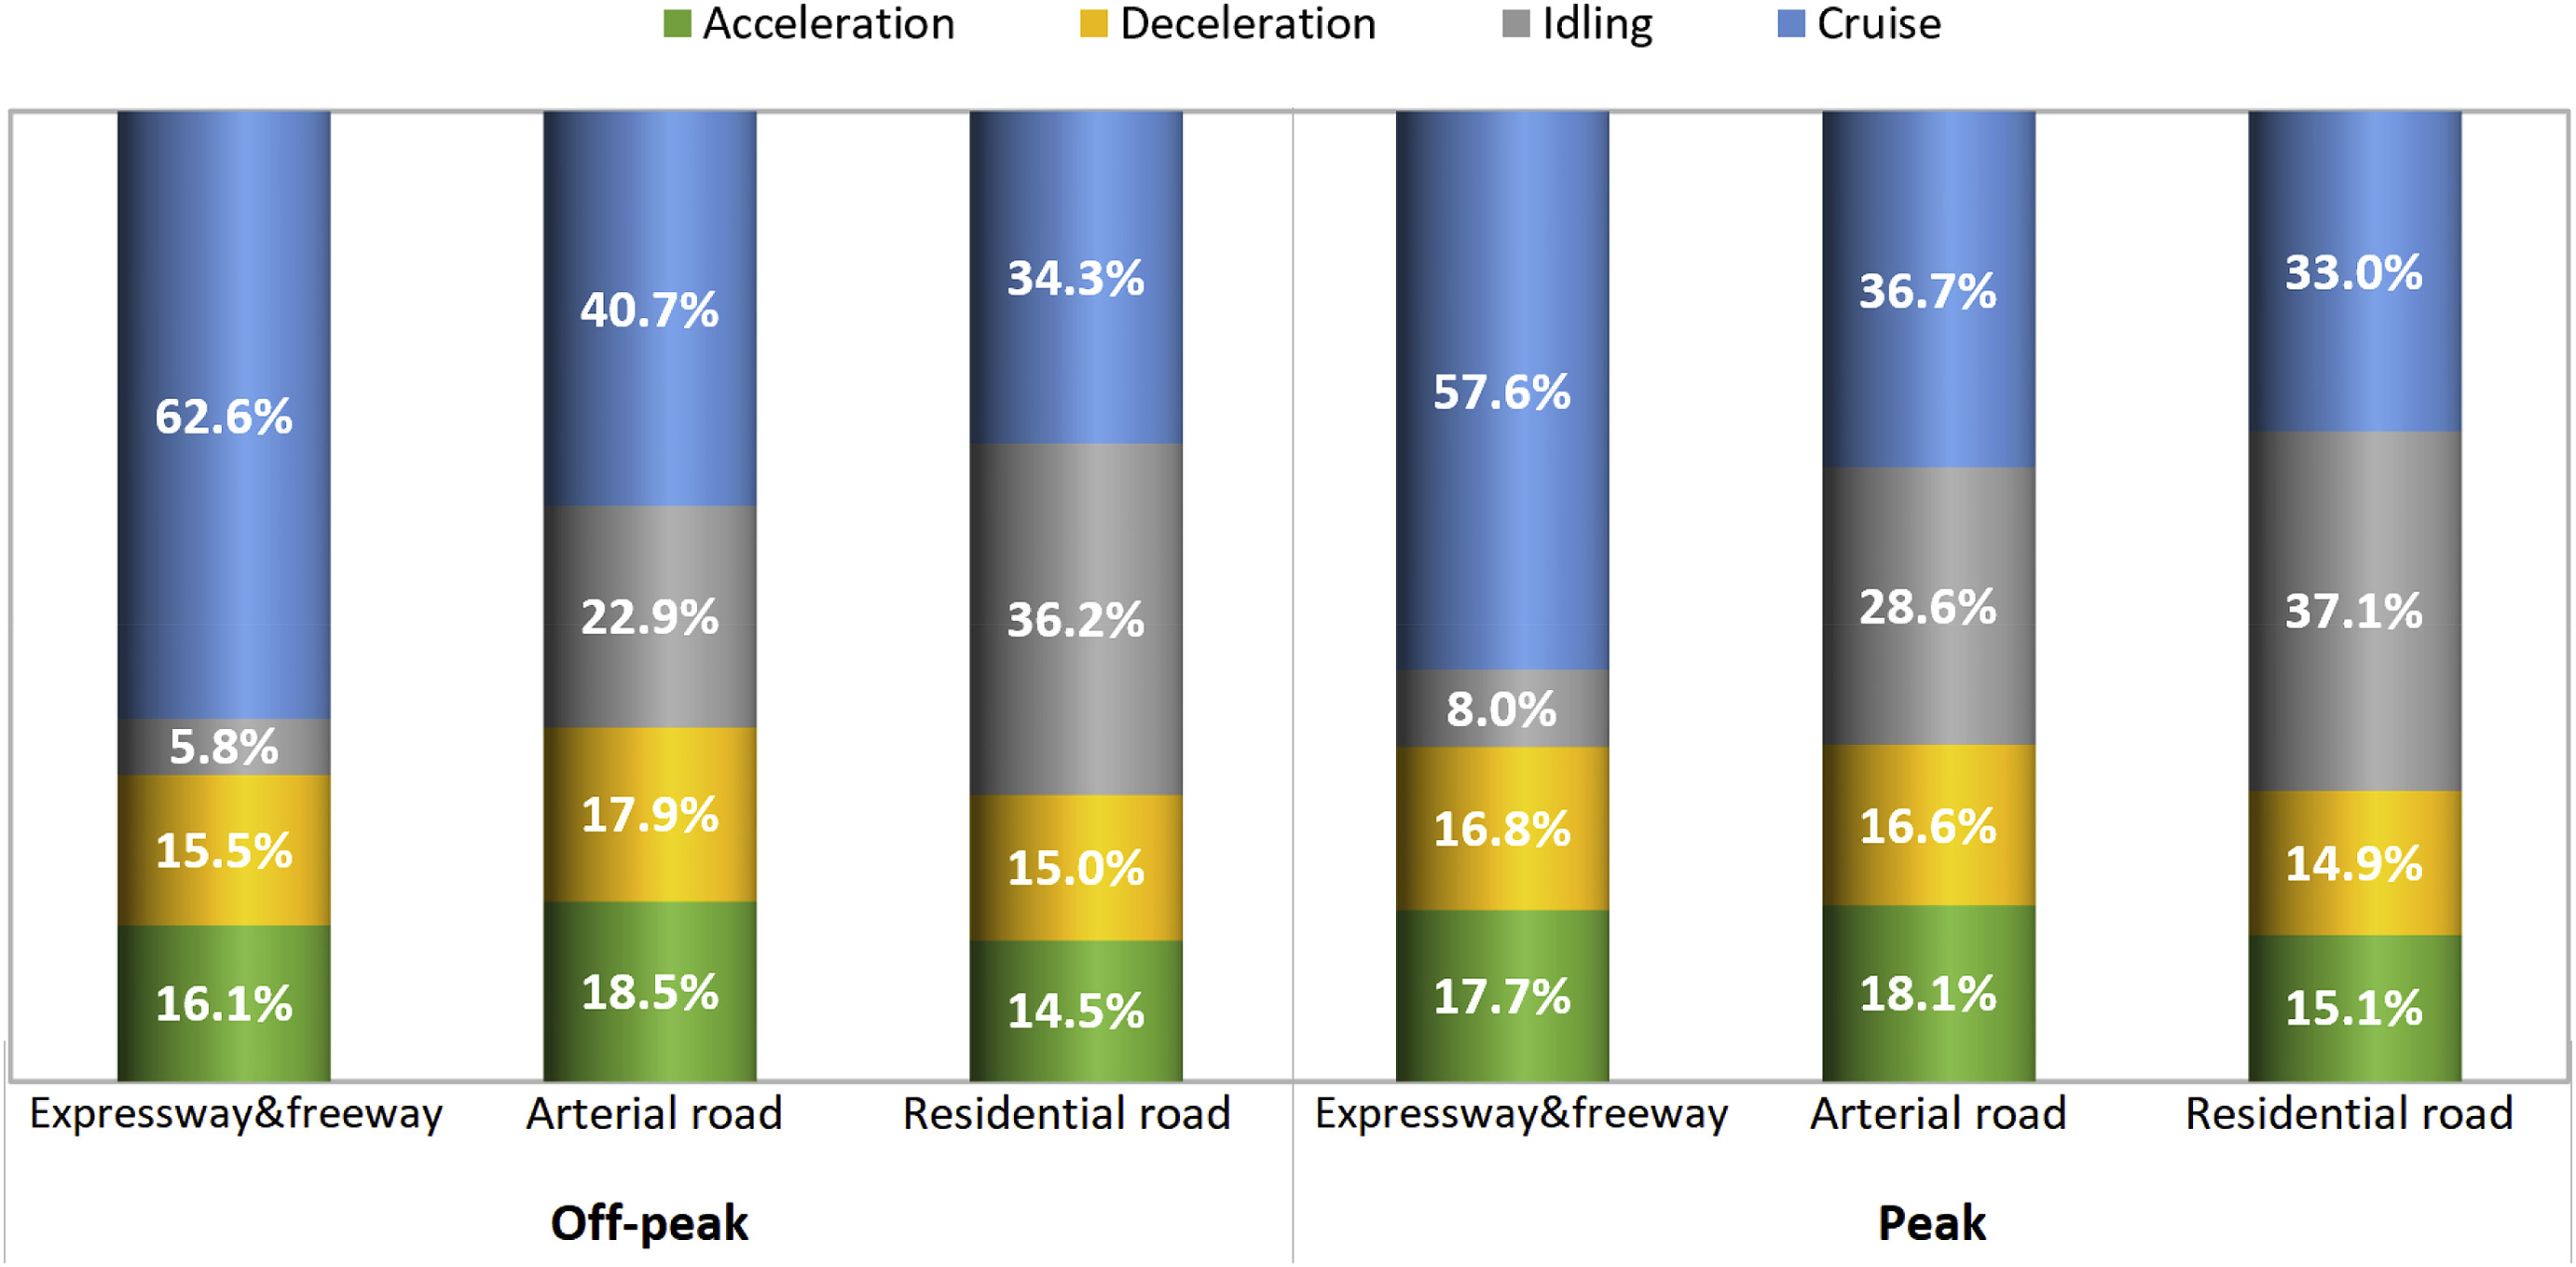
\includegraphics[width=0.7\linewidth]{Figures/ch2_shareOfDrivingModeChina.jpg}
    \caption{Proportion of driving phases during urban operation (Source: \cite{ma_real-world_2019})}
    \label{fig:ch2proportiondrivingmode}
\end{figure}

\newpage 

Most trips in Europe are short, with 80\% under 10 km and 22 minutes \cite{donati_individual_2015}, reinforcing the relevance of frequent transient phases and vehicle warm-up times, especially for Internal Combustion Engine Car (ICE). Trips powered by human effort becomes a plausible benchmark for energy use over such durations.

\begin{figure}[h!]
    \centering
    \subfloat{
        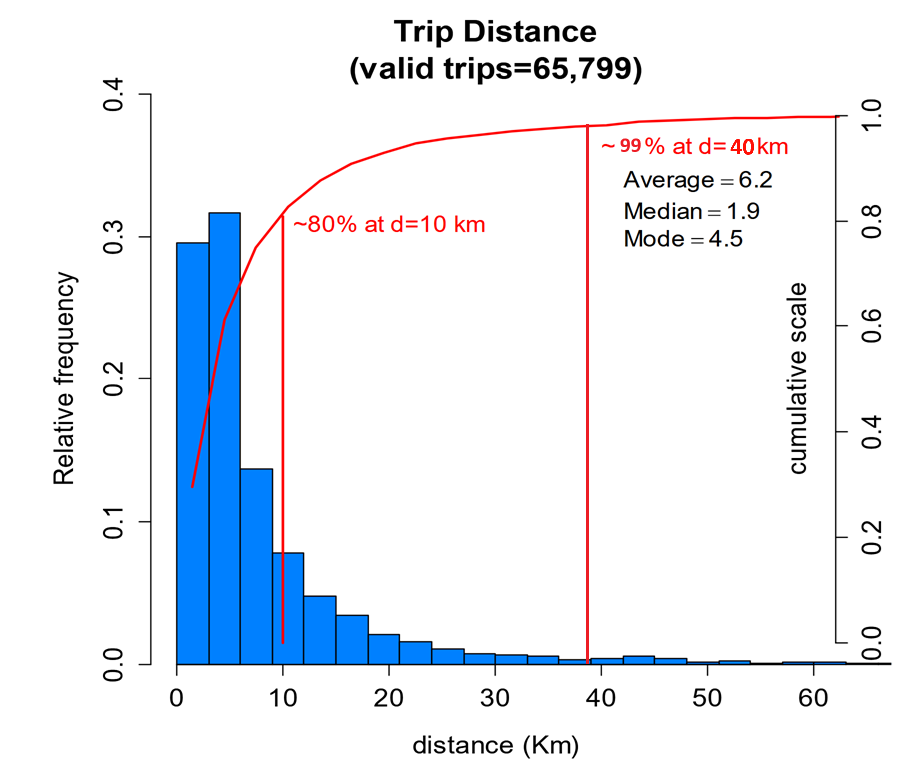
\includegraphics[width=0.45\linewidth]{Figures/ch2_TripsLenghtFrequency.png}
        \label{fig:trips-length}
    }
    \hfill
    \subfloat{
        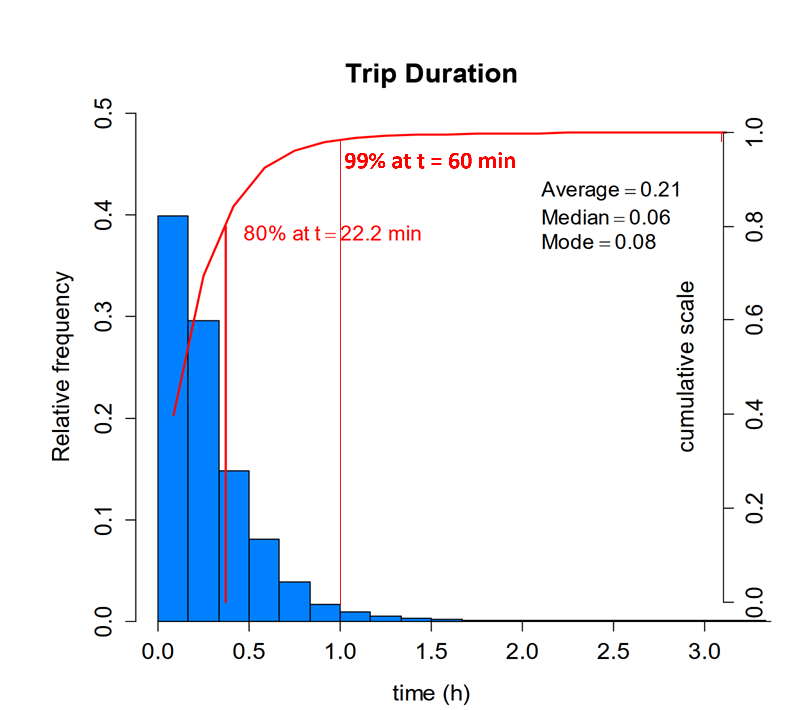
\includegraphics[width=0.45\linewidth]{Figures/ch2_TripsDurationFrequency.png}
        \label{fig:trips-duration}
    }
    \caption{Trip length and duration distributions in Europe (Source: \cite{donati_individual_2015})}
    \label{fig:trips-comparison}
\end{figure}

We define distinct phase efficiencies:

\begin{itemize}
    \item \textbf{Idling Efficiency:} Energy consumed per unit time when stationary. Typically:
    \begin{itemize}
        \item ICE: ~12 kW
        \item EV: $\leq$ 0.5 kW
    \end{itemize}

    \item \textbf{Braking/Deceleration Efficiency:} Energy recovered during braking.
    \begin{itemize}
        \item ICE: 0\%
        \item EV (regen): 50–70\% \cite{noauthor_regenerative_nodate}
    \end{itemize}

    \item \textbf{Acceleration Efficiency:} Energy transferred from tank/battery to kinetic motion.
    \begin{itemize}
        \item ICE: ~13\%
        \item EV: up to 80\% \cite{lohse-busch_ambient_2013}
    \end{itemize}
\end{itemize}

These phase-specific efficiencies reinforce the importance of designing for all driving modes, especially in urban environments characterized by frequent starts and stops.

\subsection{Embodied Energy and Material Impact: Why Mass Matters}

Although this work does not perform a full lifecycle analysis, it is important to acknowledge that manufacturing represents a non-negligible share of a vehicle’s total emissions especially for EVs with energy-intensive battery production. As grid carbon intensity decreases, manufacturing emissions become the limiting factor.

A low-mass, long-lived vehicle, built from materials with low embodied energy, offers a clear advantage in this regard.

\newpage 

\subsection{Parameters Affecting Efficiency}

From Eq.~\eqref{eq:energy_consumption}, we identify key parameters influencing operational energy efficiency:

\begin{itemize}
    \item Reduce \textbf{mass} \(m\) to minimize both rolling resistance and gravitational load.
    \item Minimize \textbf{frontal area} \(A\) and optimize \textbf{drag coefficient} \(C_d\).
    \item Lower the \textbf{rolling resistance coefficient} \(C_{rr}\) via tire selection and surface optimization.
    \item Maximize \textbf{powertrain efficiency} to reduce losses during acceleration and regenerative braking.
    \item Improve \textbf{idling efficiency}, especially critical for short, stop-start urban trips.
\end{itemize}

\subsection{Aerodynamic Optimization Through Form Factor}

Compact, narrow vehicle designs naturally limit frontal area \(A\). Reclined seating and tandem configurations can further reduce the product \(C_d A\), though this introduces challenges related to comfort and accessibility.

\begin{figure}[h!]
    \centering
    \subfloat{
        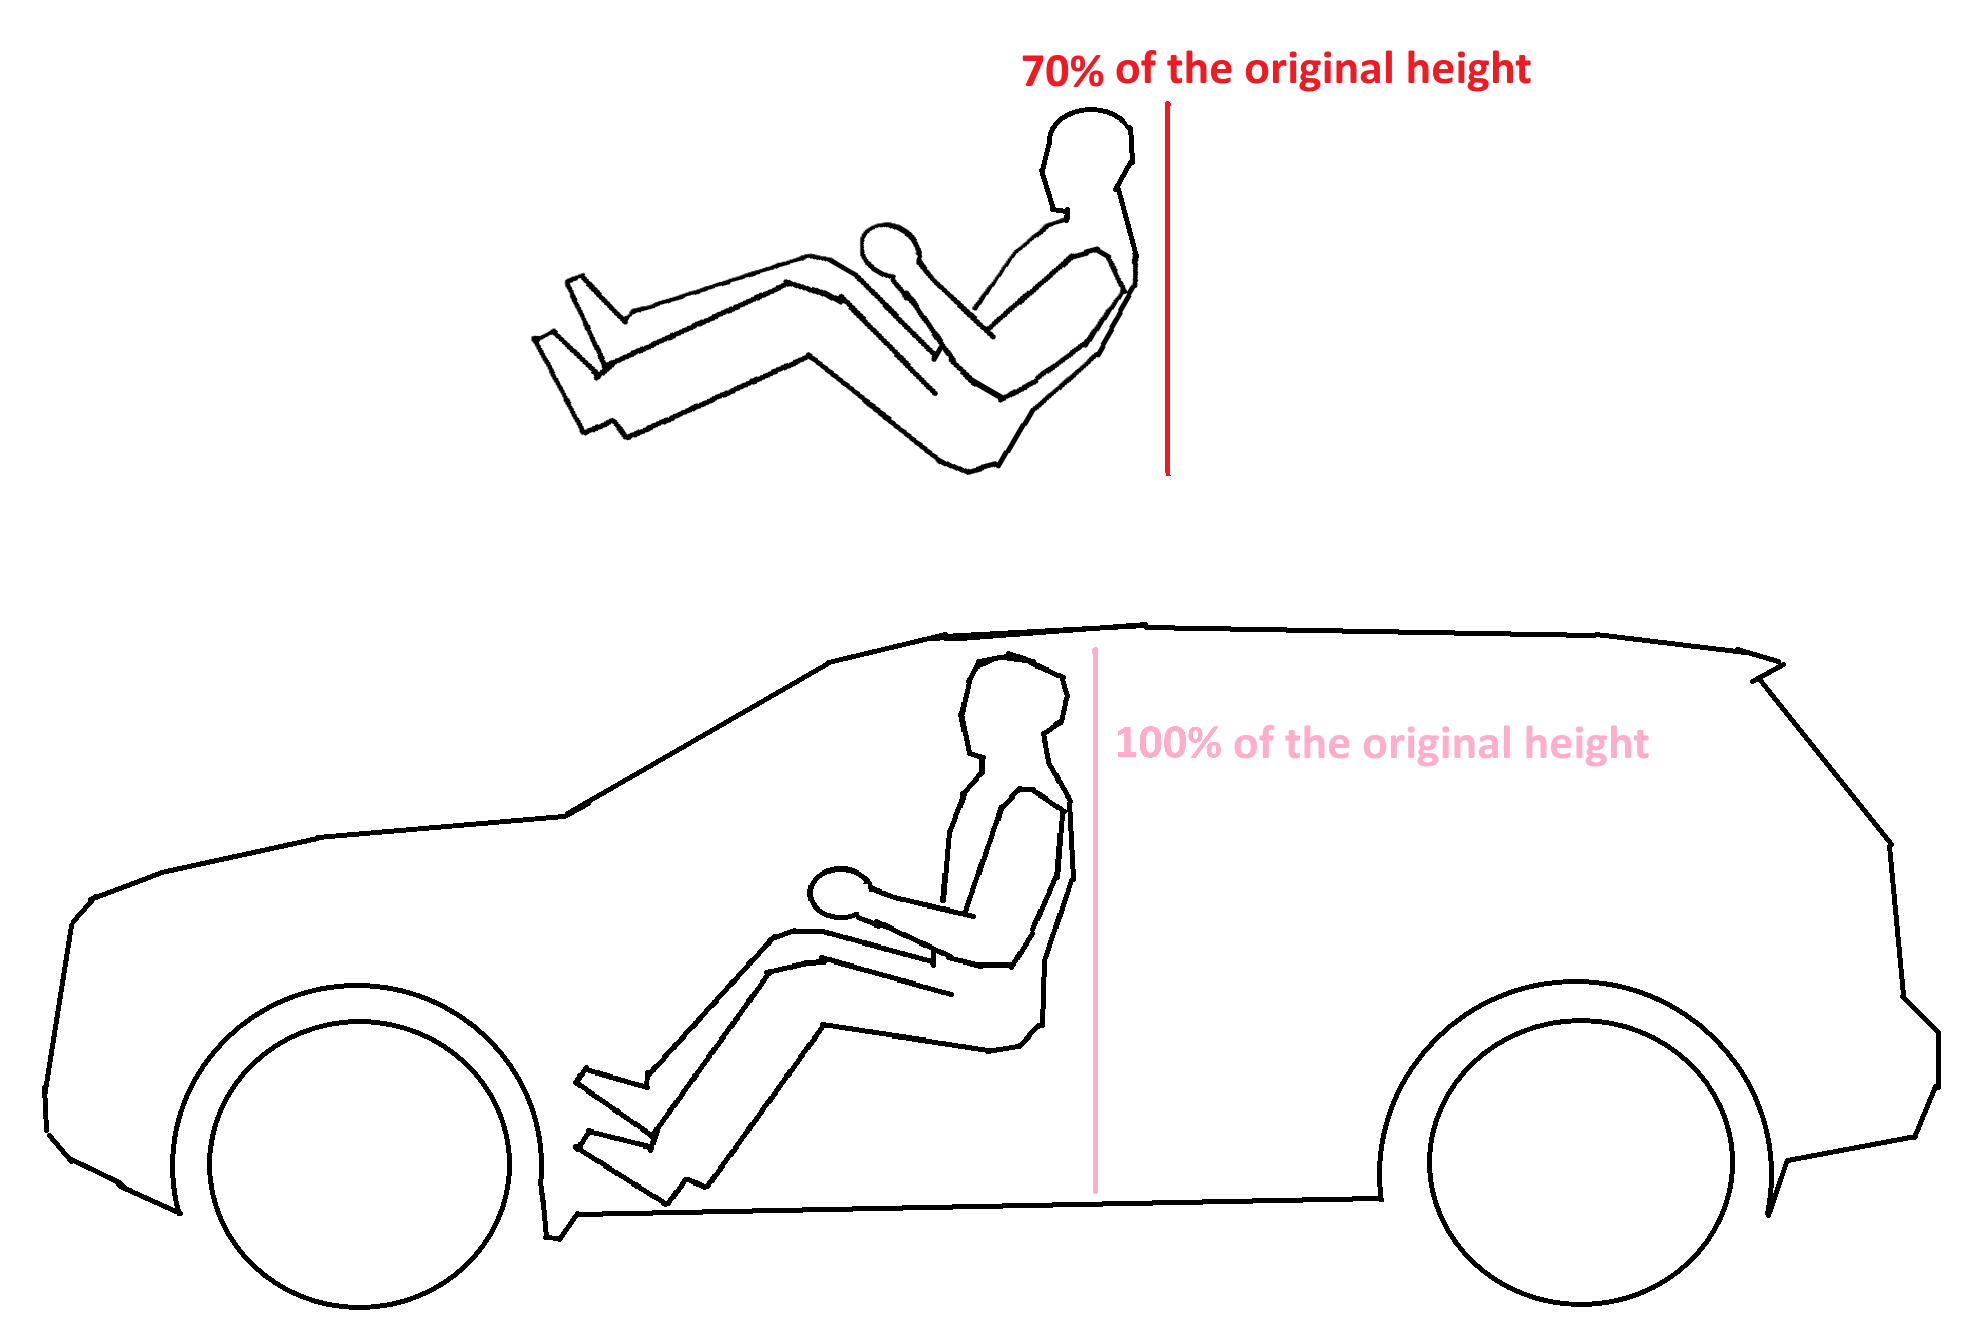
\includegraphics[width=0.47\linewidth]{Figures/ch3_seatingOptimisation.png}
    }
    \hfill
    \subfloat{
        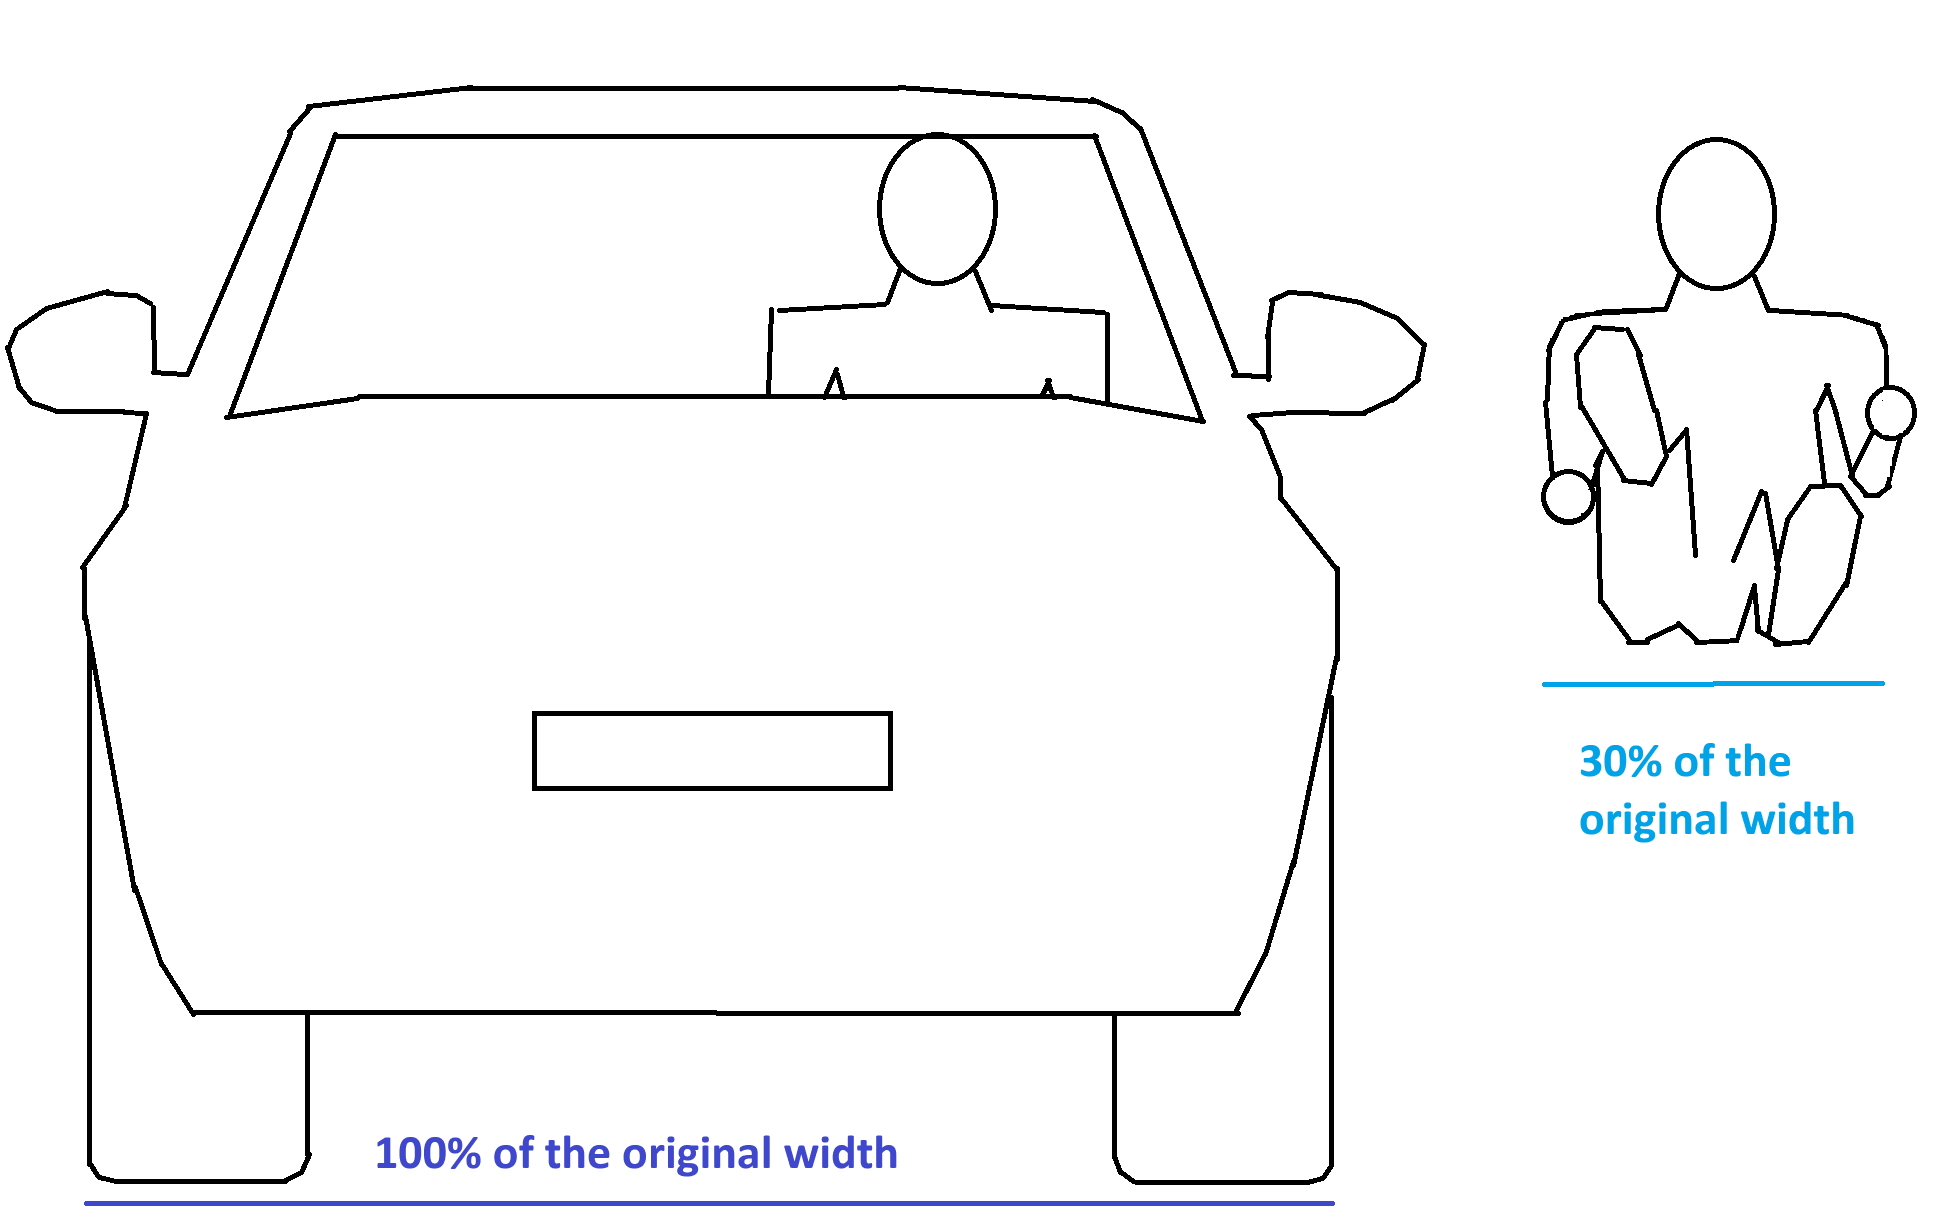
\includegraphics[width=0.47\linewidth]{Figures/ch3_seatingOptimisationFront.png}
    }
    \caption{Effect of seat recline and tandem seating on frontal area}
    \label{fig:FrontaAreaGraphicsComparison}
\end{figure}

Digital augmentation (cameras, screens) could replace traditional visibility elements to further reduce \(A\), but may induce motion sickness due to visual-vestibular mismatches. A partially reclined posture with direct external visibility is a pragmatic compromise.

\begin{figure}[h!]
    \centering
    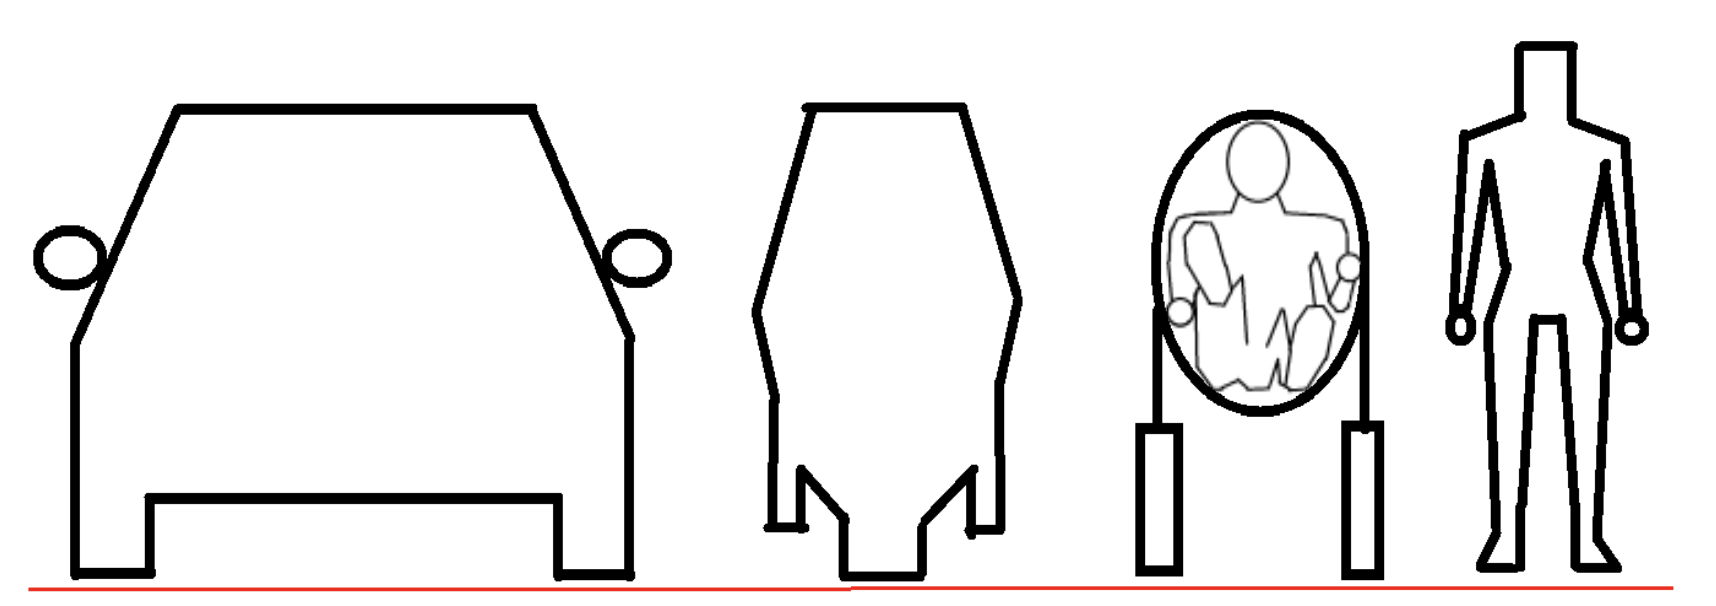
\includegraphics[width=0.8\linewidth]{Figures/ch4_frontComparisonVehicle.png}
    \caption{Frontal area comparison of car, leaning vehicle, proposed concept, and a standing person}
    \label{fig:frontal_comparison}
\end{figure}

Our proposed design incorporates a height-adjustable wheel system, enabling both dynamic tilt control and variable ingress/egress configurations combining aerodynamic form with accessibility.

